\documentclass{article}

\usepackage{tgbonum}    % Tex Gyre Bonum
% \usepackage{mathptmx} % Times New Roman

% Header
\usepackage{fancyhdr}
\pagestyle{fancy}
\lhead{Daniel Jahn}
\rhead{Spatio-temporal clustering}
\cfoot{\thepage}
\renewcommand{\headrulewidth}{0.4pt}

% Images
\usepackage{graphicx}
\graphicspath{ {Images/} }

% Bibliography
\usepackage{natbib}
\bibliographystyle{unsrtnat}


% Todonotes
\usepackage{xargs} % For definining new todonotes
\usepackage[prependcaption,textsize=tiny]{todonotes} % disable
\newcommandx{\problem}[2][1=]{\todo[linecolor=red,backgroundcolor=red!25,bordercolor=red,#1]{#2}}
\newcommandx{\todoo}[2][1=]{\todo[linecolor=blue,backgroundcolor=blue!25,bordercolor=blue,#1]{#2}}
\newcommandx{\note}[2][1=]{\todo[linecolor=OliveGreen,backgroundcolor=OliveGreen!25,bordercolor=OliveGreen,#1]{#2}}
\newcommandx{\unsure}[2][1=]{\todo[linecolor=Plum,backgroundcolor=Plum!25,bordercolor=Plum,#1]{#2}}


% Mathematical symbols
\usepackage{amsmath}
\usepackage{amssymb}


% Options for the caption font
\usepackage[font=small]{caption}





\begin{document}

% Article top matter
\title{NMST543 \\
Spatio-temporal clustering}
\author{Daniel Jahn \\
jahn@karlin.mff.cuni.cz}  
\date{\today} 
\maketitle


\section{Introduction}

\section{Interaction and clustering}
In order to understand the term \textit{spatio-temporal clustering}, care has to be taken to carefully tease apart the related concepts of interaction and clustering.

We distinguish between spatial and temporal clustering. \textbf{Spatial clustering} results in the inhomogeneity of spatial distribution. An example is the crime rate being higher in densely populated areas. 
\textbf{Temporal clustering} results in the inhomogeneity of temporal distribution. An example are seasonal trends, such as an increased incidence of disease during winter. 
 
Interaction is typically understood to be a mechanism through which the location of one or more points influences the locations of others. For example, certain tree species prefer to grow further from other trees, thus resulting in repulsion between the individual locations. In the temporal domain, we have e.g. the refractory period for neurons, where one neuron remains inactive for a small period after firing. 

Both interaction and clustering result in inhomogeneity of the point patterns. From a statistical perspective, their difference is often purely interpretational, as they cannot distinguished through data only, but require domain knowledge to interpret the origin of the inhomogeneity. 

These two terms blur together somewhat when we deal with data with both spatial and temporal component. A mere presence of both spatial and temporal clustering do not suffice for spatio-temporal clustering in the sense of the word as used in \cite{diggle1995}. They give an example of a disease, which may cluster in densely populated areas and be more prevalent during cold weather. However, the disease only manifests spatio-temporal clustering if it is contagious.
This is reflected in the fact that the terms interaction and clustering are used interchangeably in the paper.



\section{Description of the method}
In this text, we investigate the spatio-temporal clustering method proposed in \cite{diggle1995}. Let $X$ be a \textbf{stationary} simple spatio-temporal point process on $\mathbb R^2\times \mathbb R$. We only observe the events $X\cap(W\times [0,T]),$ where $W$ is bounded Borel with $|W|>0$ and $T>0$. We define its projections to the spatial and temporal domain,
$$X_1 = \{x \in W: (x,t)\in X\cap (W\times [0,T])\}, \quad X_2 = \{t \in [0,T]: (x,t) \in X\cap (W\times [0,T])\},$$
and we assume $X_1$ and $X_2$ to be simple. We denote the intensity of $X$ by $\lambda$ and the intensities of $X_1$ and $X_2$ by $\lambda_1$ and $\lambda_2$, respectively. Note that $\lambda_1 = \lambda T$ and $\lambda_2 = \lambda |W|$.


We utilize the \textit{K-function}, which can be defined by
$$\lambda K(s,t) = \mathrm{E} \sum^{\neq}_{(x,t_1),(y,t_2)\in X} \frac{1_A(x) 1_{[0,s]}(\|x-y\|) 1_S(t_1) 1_{[0,t]}(|t_1 - t_2|)}{\lambda |A| |S|}$$
where $A \subset \mathbb R^2, S \subset \mathbb R$ are arbitrary Borel sets with finite and positive measure. We can interpret the term $\lambda K(s,t)$ as the number of further events occurring within distance $s$ and time $t$ of an arbitrary event.

Under the assumption of spatio-temporal independence, i.e. the independence of $X_1$ and $X_2$, we obtain the factorization
$$K(s,t)=K_1(s)K_2(t),$$
where $K_1$ and $K_2$ are the \todoo{Not really defined}K-functions of $X_1$ and $X_2$, respectively. Analogously, their interpretation is the number of further events occurring withing distance $s$, respectively within time $t$, of an arbitrary event.

The K-functions serve as a basis for the method proposed by \cite{diggle1995}. The functions $K,K_1,K_2$ will be used not only for testing for spatio-temporal interaction, but also to measure the extent and nature of it.

\subsubsection{Estimates}

Let $\{(x_i,t_i): i=1,\dots, n\}$ denote the locations and times of all events within $W\times [0,T]$. We introduce the estimates
$$\hat K(s,t) = |A|T (n(n-1))^{-1} \sum_{j\neq i} w_{ij} v_{ij} I_{[d_{ij} \leq s]} I_{[u_{ij} \leq t]},$$	
$$\hat K_1(s) = |A| (n(n-1))^{-1} \sum_{j\neq i} w_{ij}  I_{[d_{ij} \leq s]},$$	
$$\hat K_2(t) = T (n(n-1))^{-1} \sum_{j\neq i}  v_{ij}  I_{[u_{ij} \leq t]},$$
where $d_{ij} = \|x_i - x_j\|$ and $u_{ij} = |t_i - t_j|$, and $w_{ij}$ and $v_{ij}$ are edge-effect corrections.


We now introduce the three visual diagnostics which can be used to describe the extent and nature of the spatio-temporal interaction.

\subsubsection{Diagnostic surface plot}


$$\hat D(s,t) = \hat K(s,t) - \hat K_1(s) \hat K_2(t)$$

\subsubsection{Residual plot}



\subsubsection{Monte-Carlo test}





Interpretation


Intractable distribution. MC test.



\section{Simulated data}


\begin{figure}[p]
  \centering
    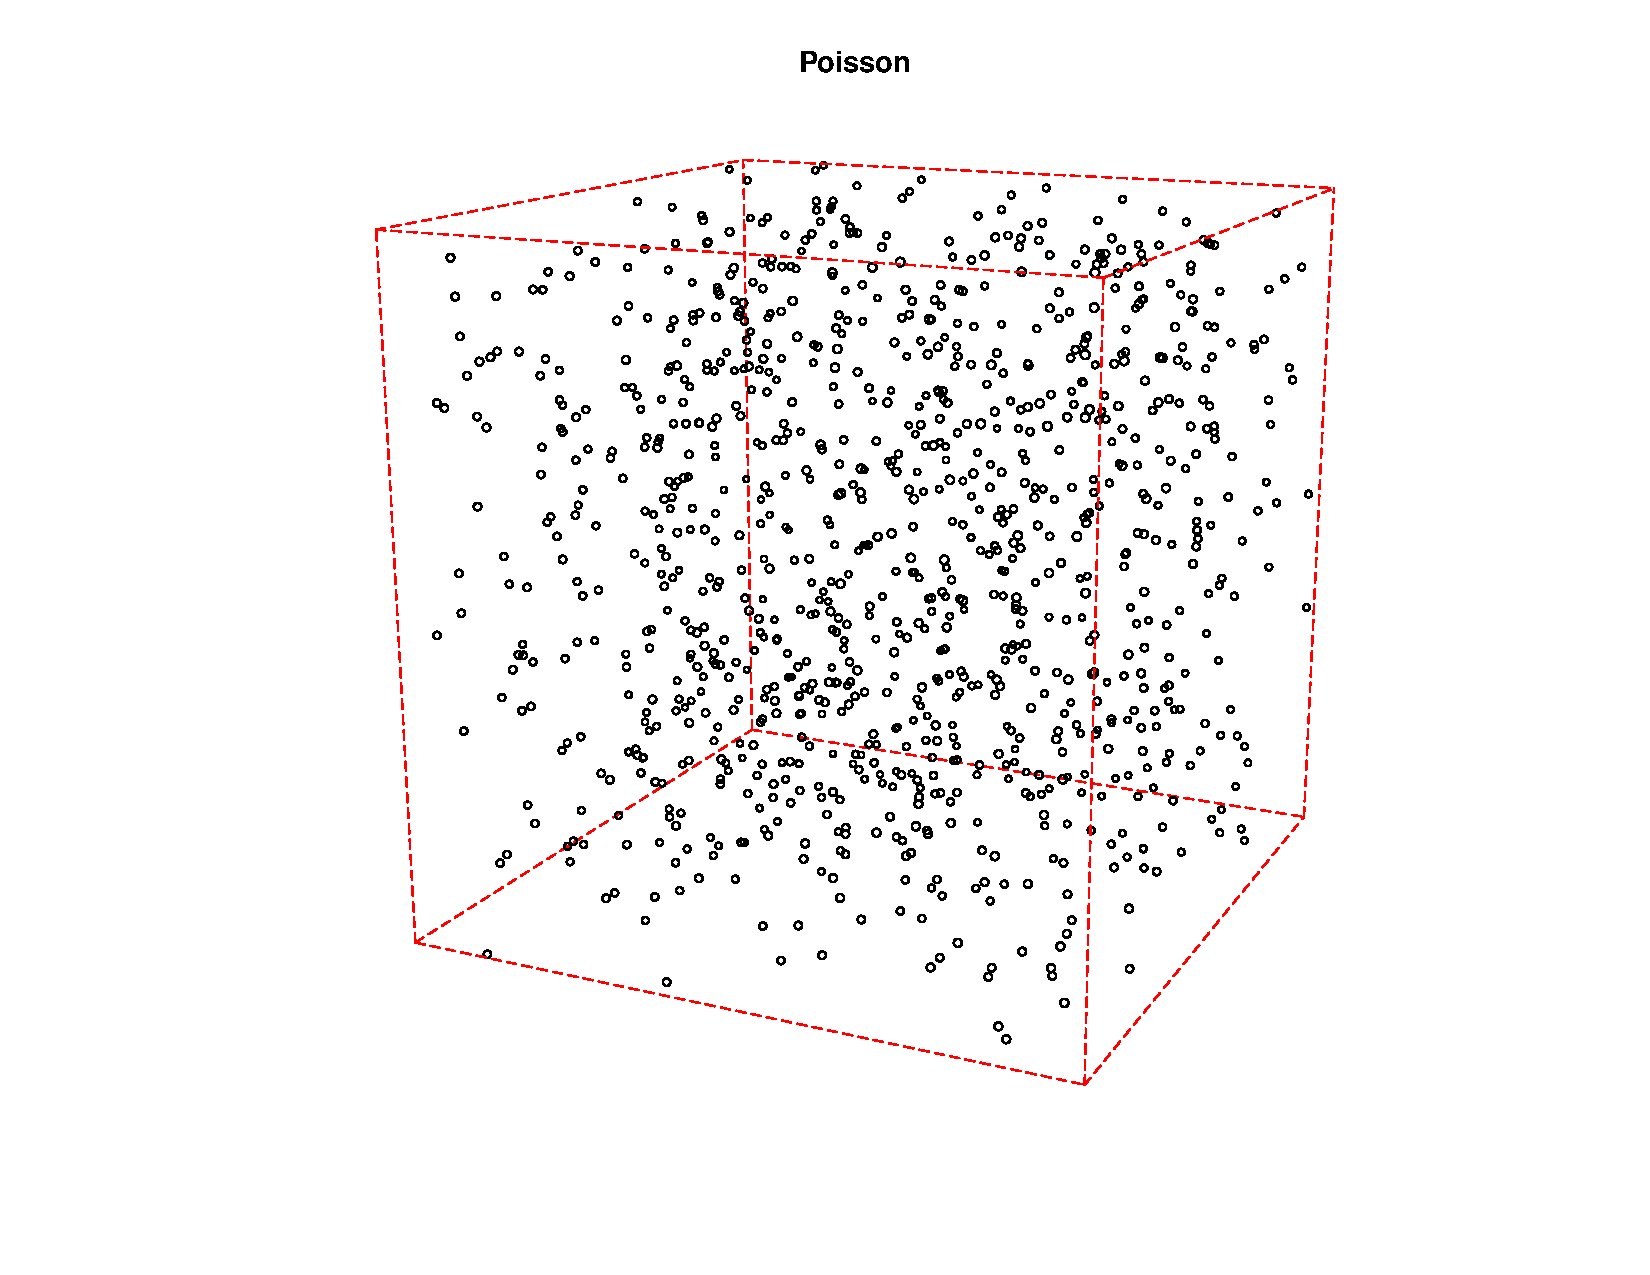
\includegraphics[width=0.9\textwidth]{PP_Poisson_1000_1021.pdf}
  \caption{Realization of a Poisson point process. Intensity . Number of points: 1021}
  \label{fig:poissonPP}


	\vspace*{\floatsep}

    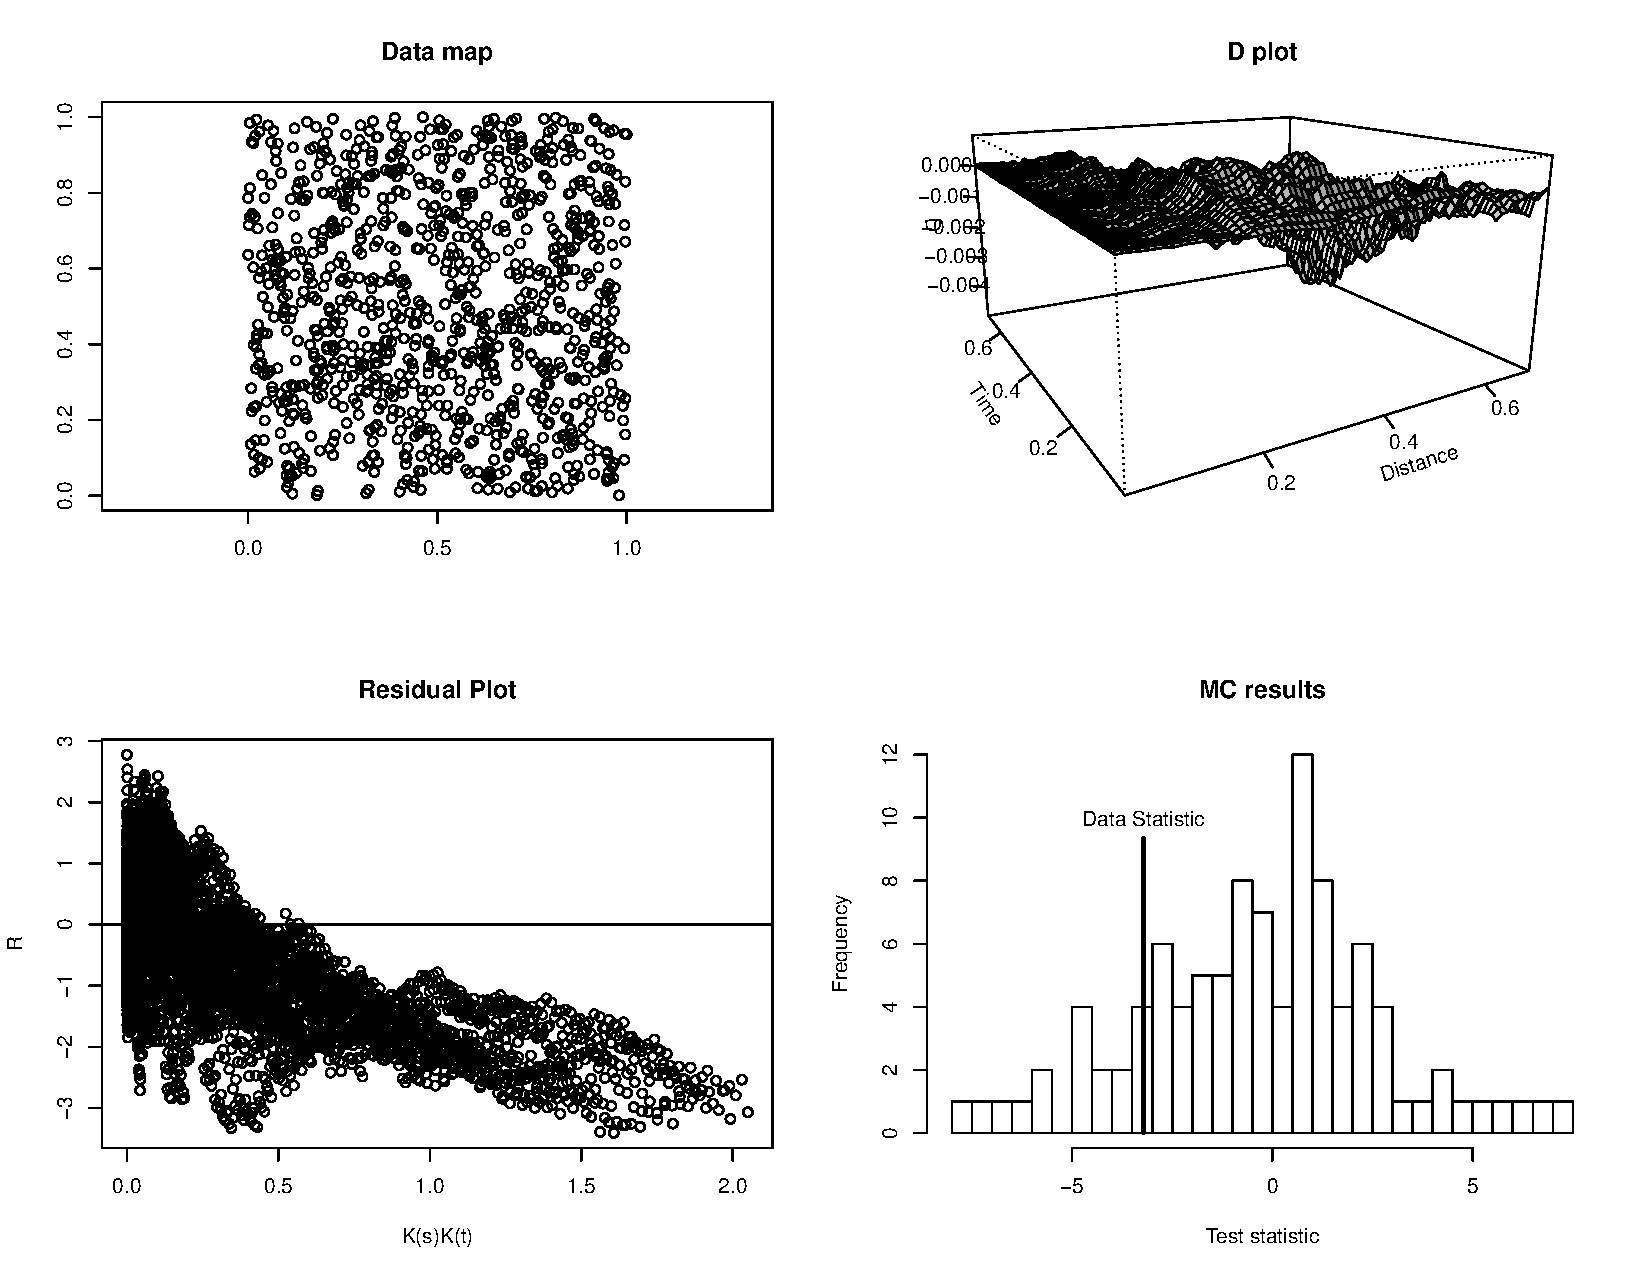
\includegraphics[width=0.9\textwidth]{diag_Poisson_1000_1021.pdf}
  \caption{Diagnostic plots for a realization of a Poisson point process. Intensity . Number of points: 1021}
  \label{fig:poissonDiag}
\end{figure}


\begin{figure}[p]
  \centering
    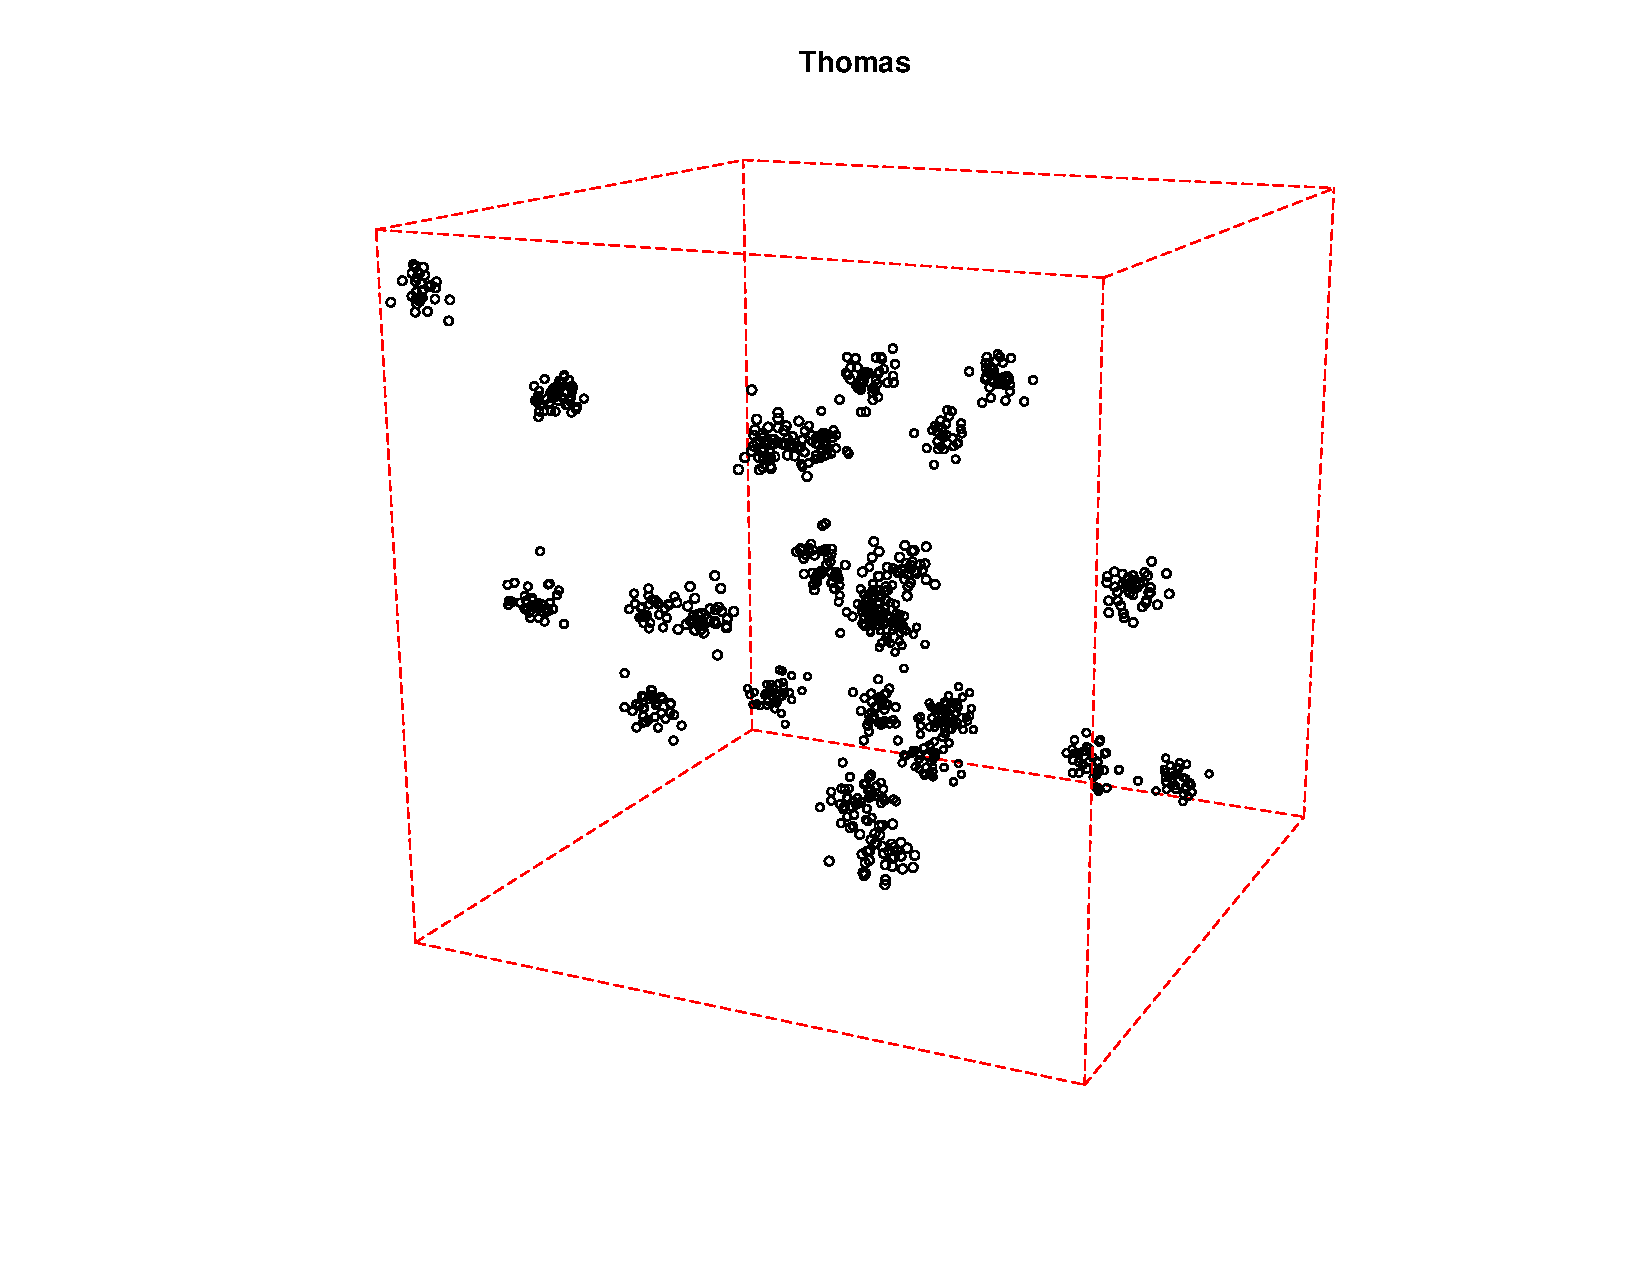
\includegraphics[width=0.9\textwidth]{PP_Thomas_20_40_0p02_949.pdf}
  \caption{Realization of a Thomas point process. Intensity of parent process 20. Child process: intensity 40, distribution $N(0,0.02)$. Number of points: 949.}
  \label{fig:thomasPP}

\vspace*{\floatsep}

    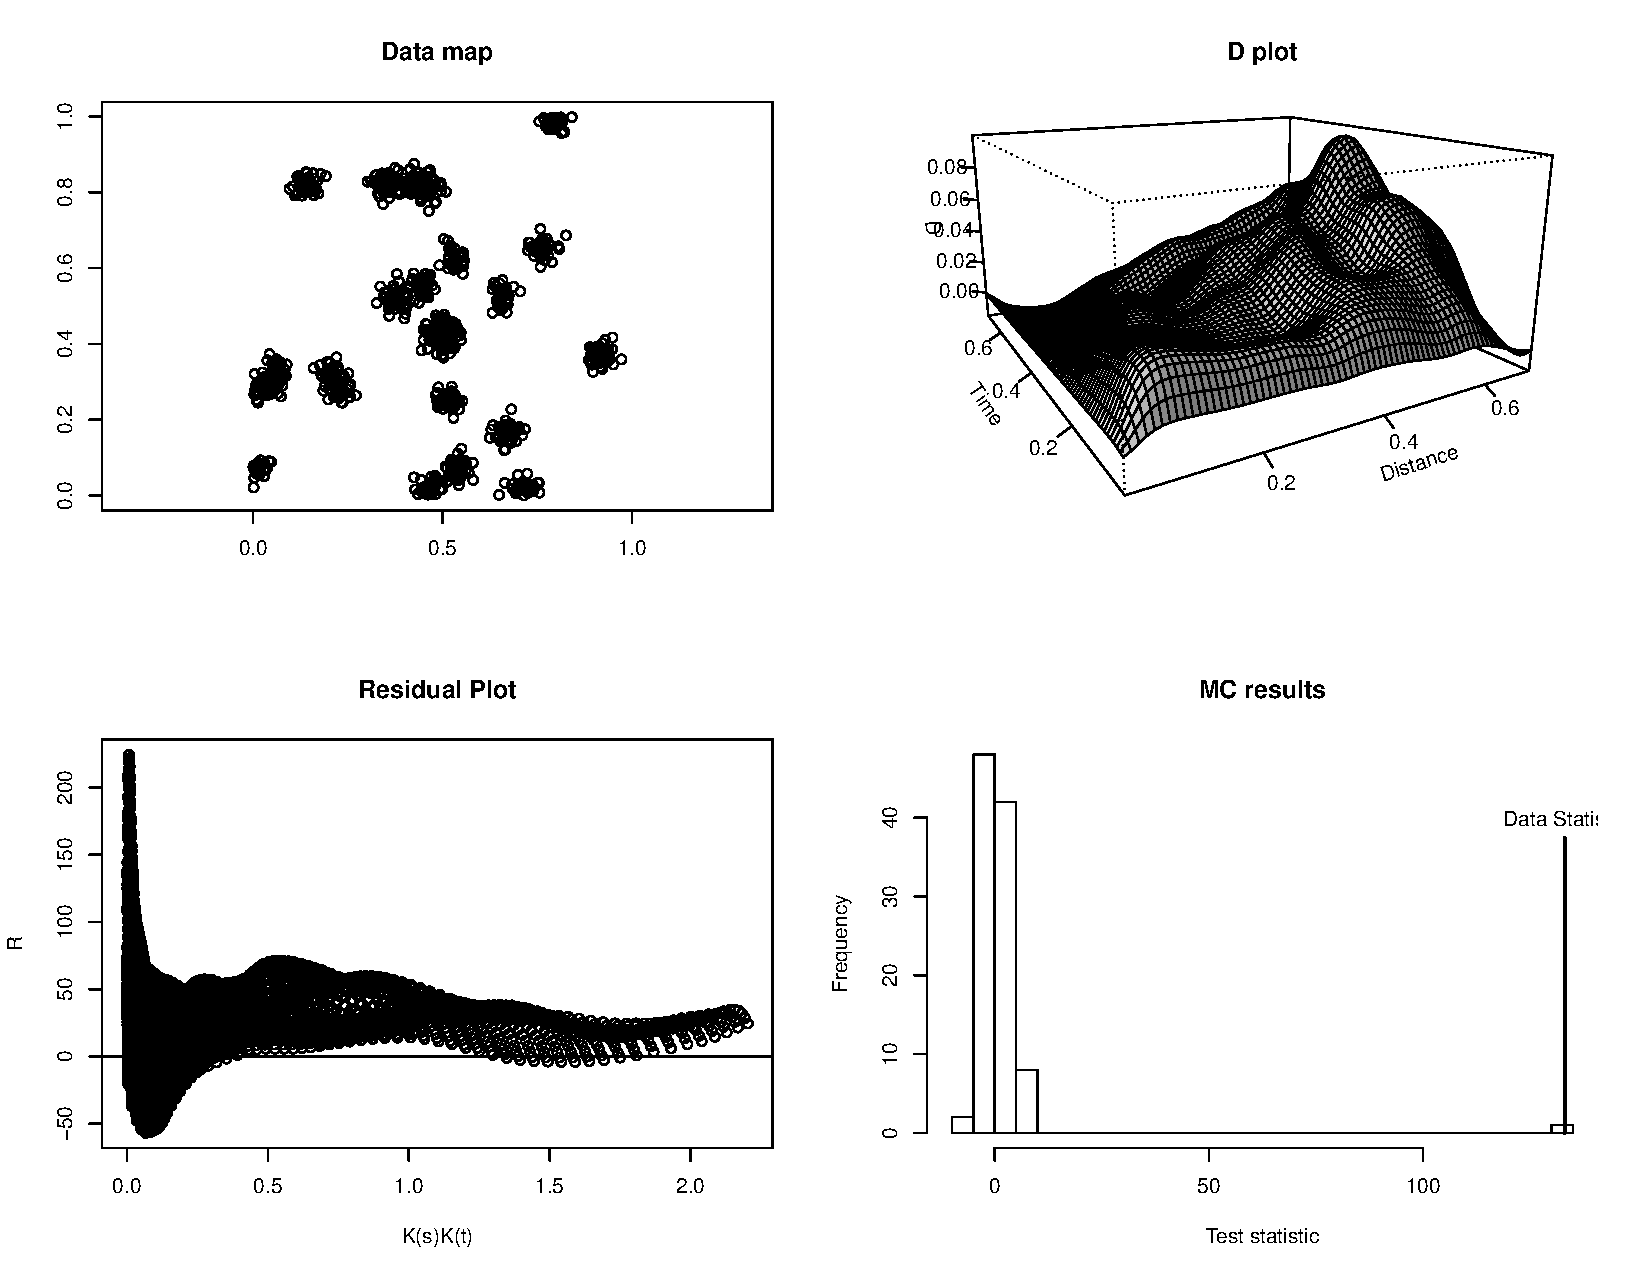
\includegraphics[width=0.9\textwidth]{diag_Thomas_20_40_0p02_949.pdf}
  \caption{Diagnostic plots for a realization of a Thomas point process. Intensity of parent process 20. Child process: intensity 40, distribution $N(0,0.02)$. Number of points: 949.}
  \label{fig:thomasDiag}
\end{figure}


\begin{figure}[p]
  \centering
    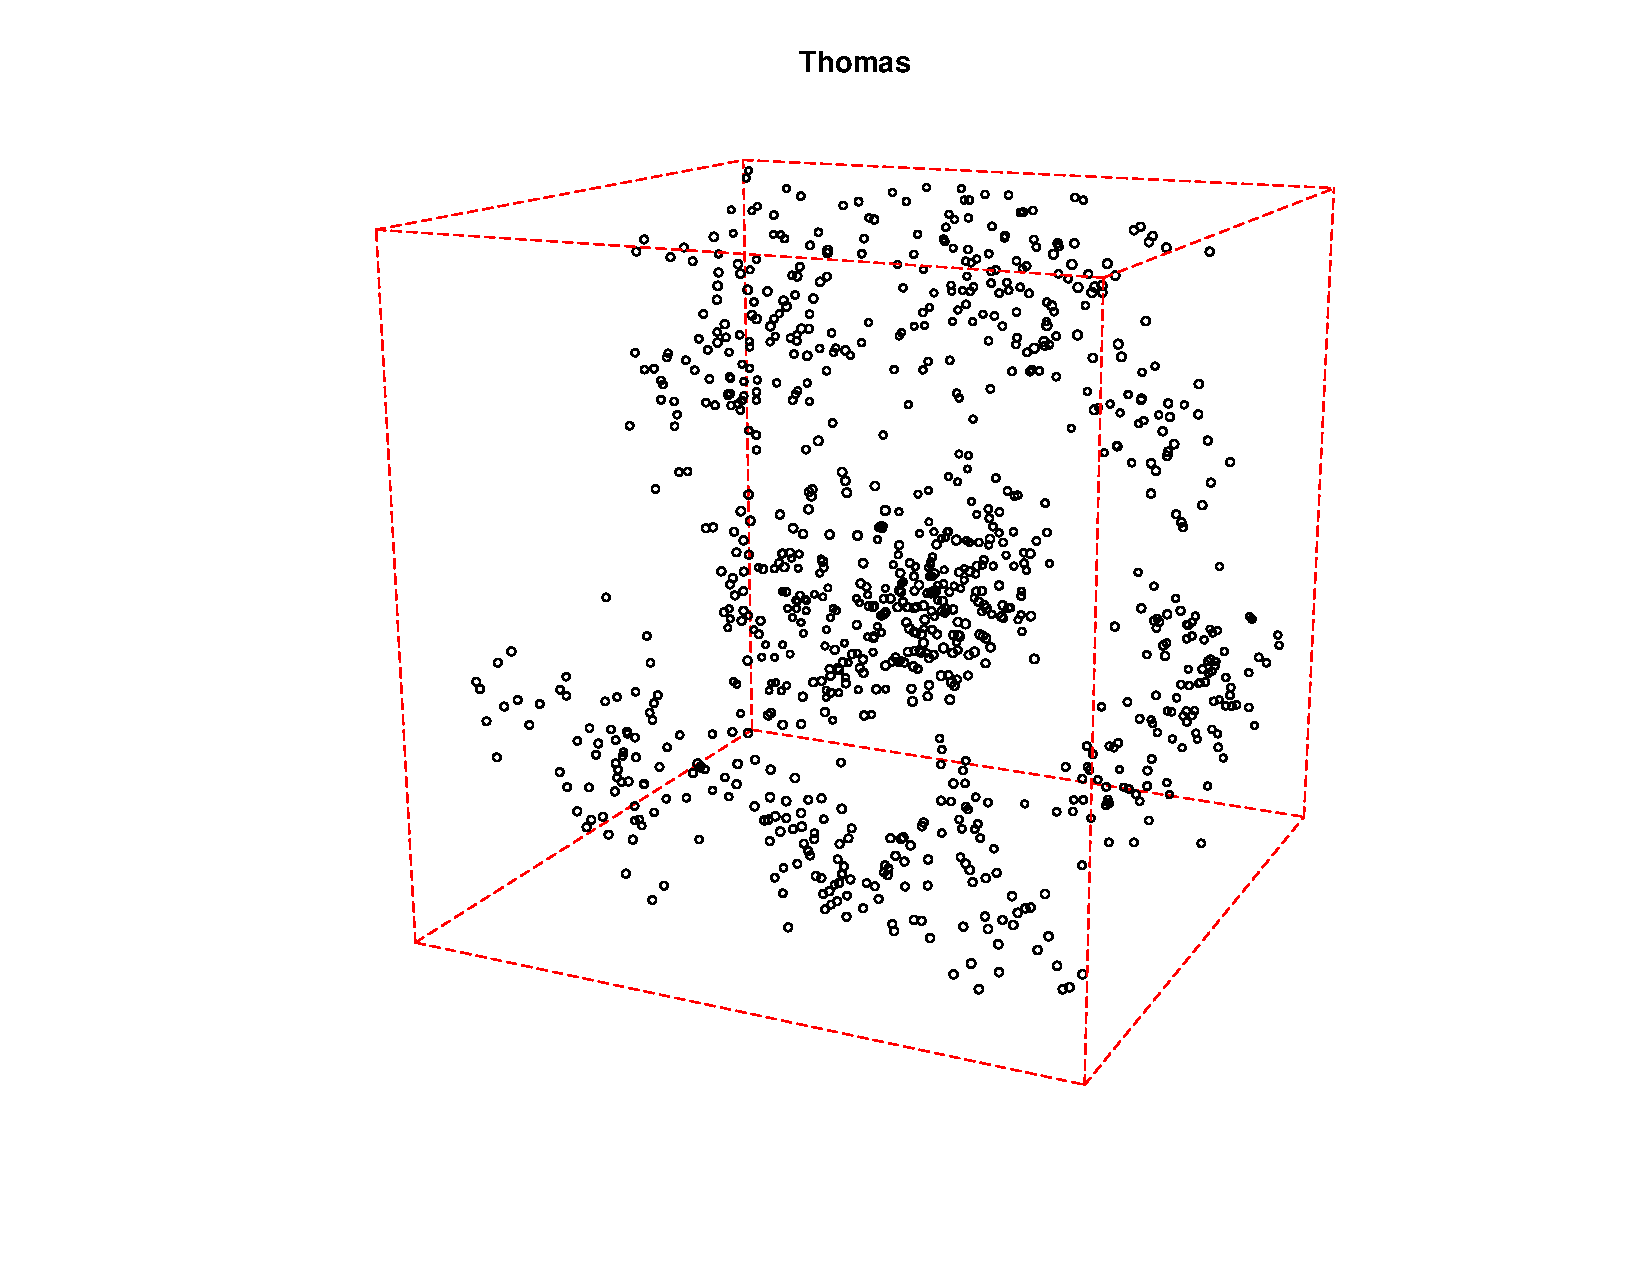
\includegraphics[width=0.9\textwidth]{PP_Thomas_40_20_0p05_929.pdf}
  \caption{Realization of a Thomas point process. Intensity of parent process 40. Child process: intensity 20, distribution $N(0,0.05)$. Number of points: 929.}
  \label{fig:thomas2Diag}

\vspace*{\floatsep}

    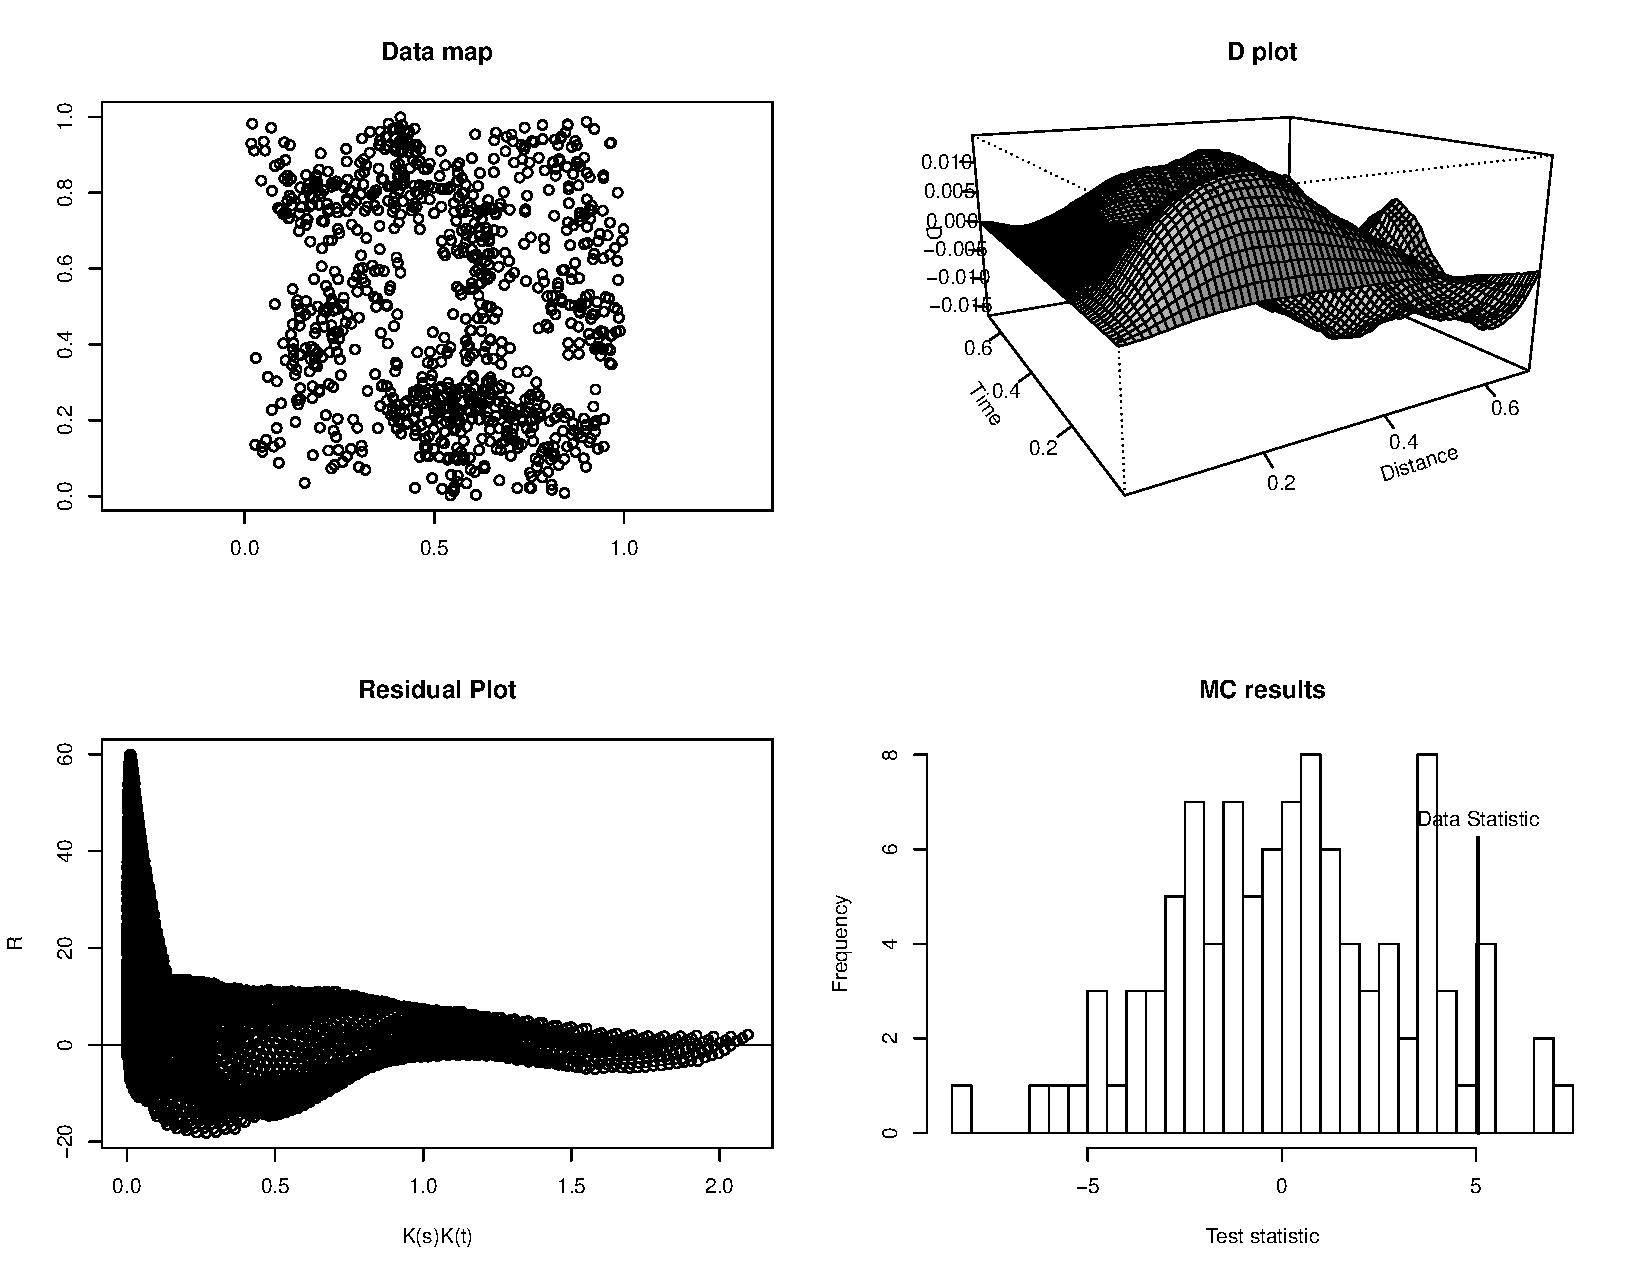
\includegraphics[width=0.9\textwidth]{diag_Thomas_40_20_0p05_929.pdf}
  \caption{Diagnostic plots for a realization of a Thomas point process. Intensity of parent process 40. Child process: intensity 20, distribution $N(0,0.05)$. Number of points: 929.}
  \label{fig:thomas2Diag}
\end{figure}



\begin{figure}[p]
  \centering
    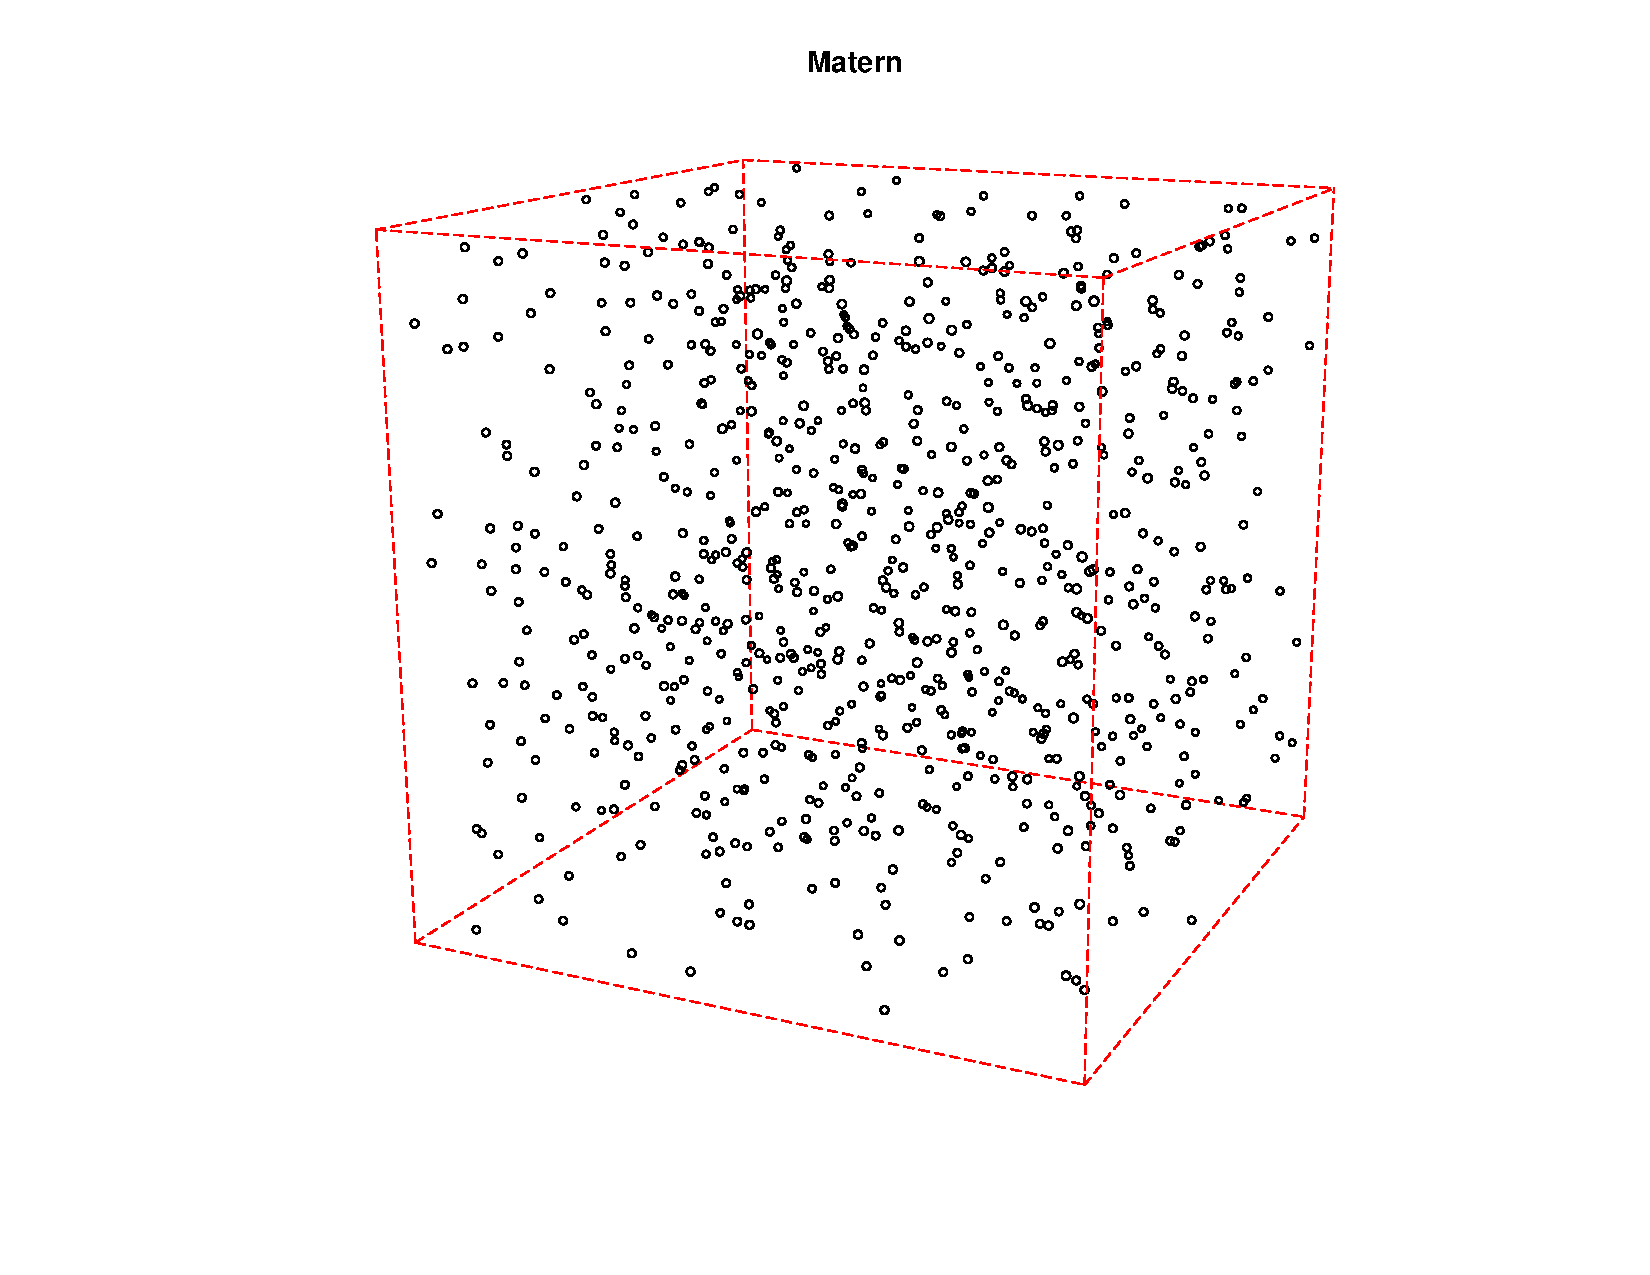
\includegraphics[width=0.9\textwidth]{PP_Matern_II_1000_0p05_818.pdf}
  \caption{Realization of a Matern II point process. Intensity 1000. Minimum distance 0.05. Number of points: 818.}
  \label{fig:maternPP}

\vspace*{\floatsep}

    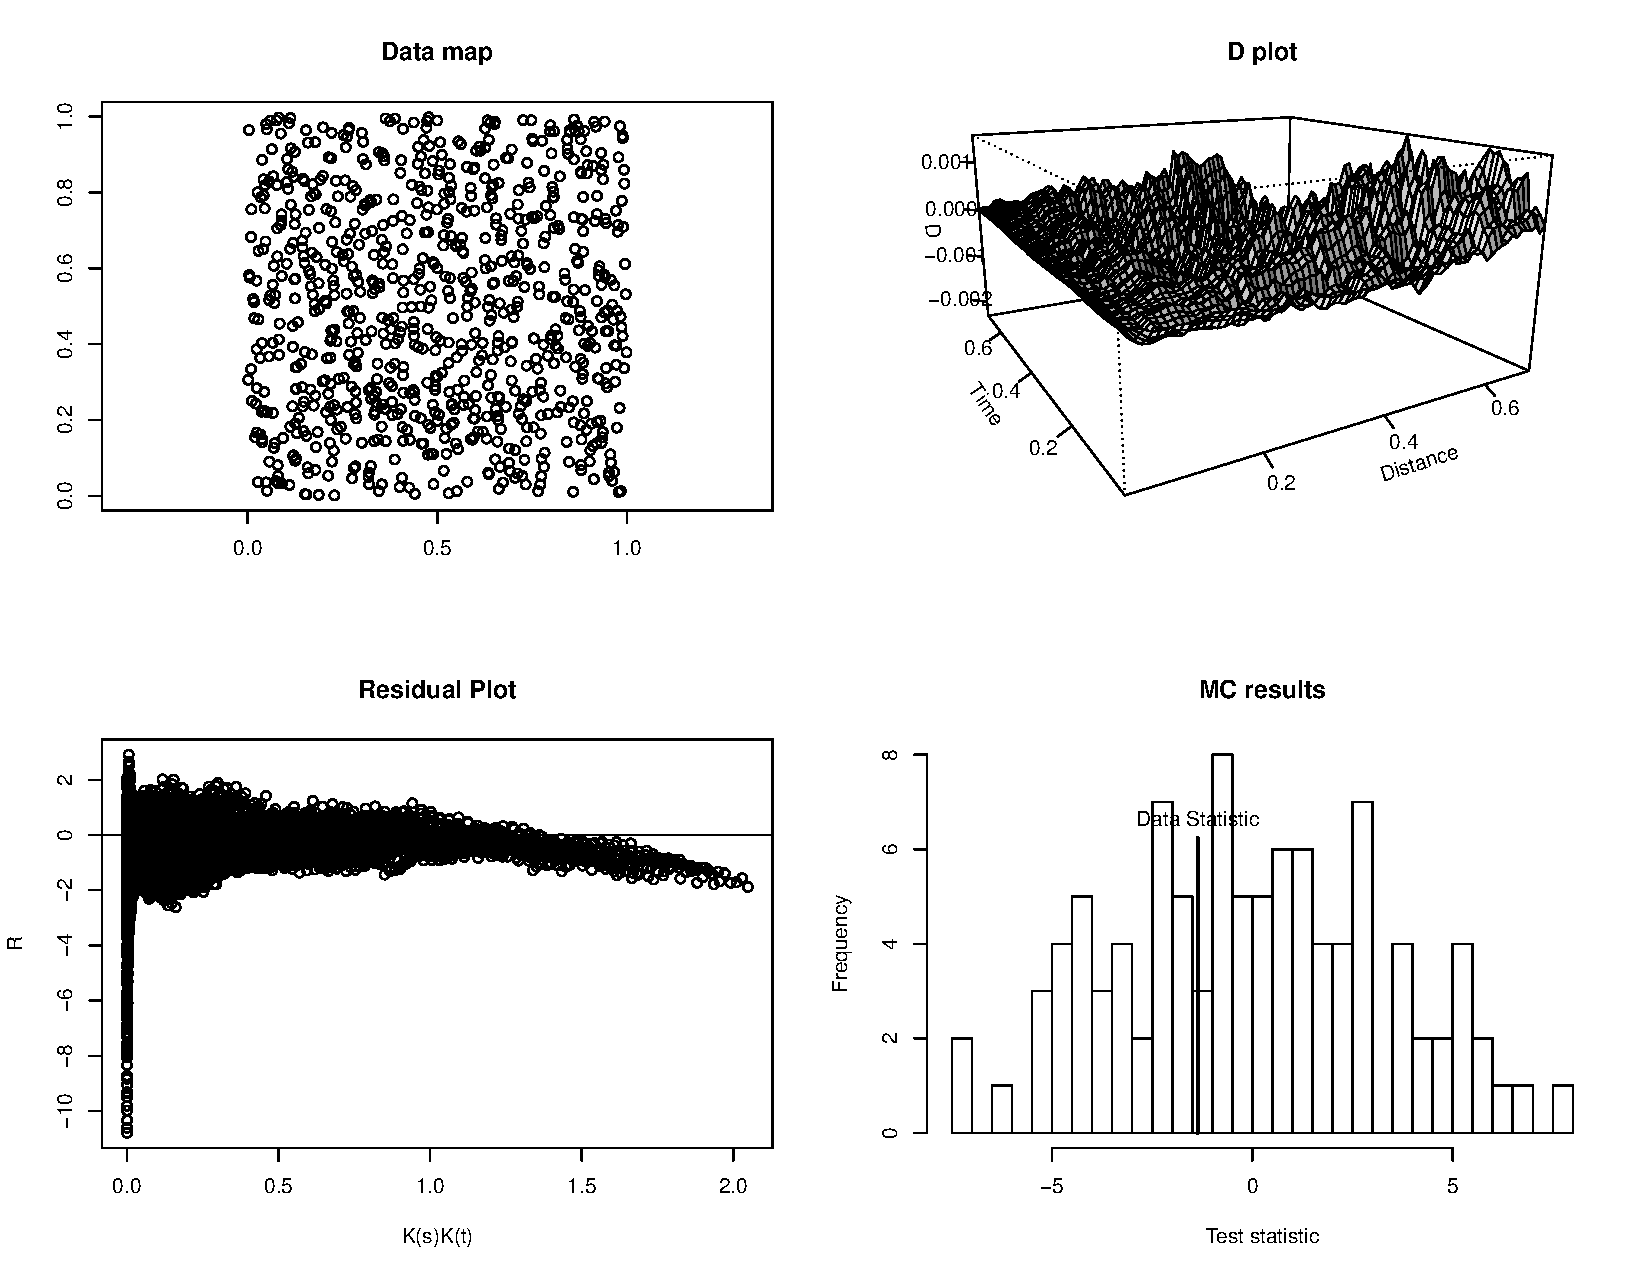
\includegraphics[width=0.9\textwidth]{diag_Matern_II_1000_0p05_818.pdf}
  \caption{Diagnostic plots for a realization of a Matern II point process.  Intensity 1000. Minimum distance 0.05. Number of points: 818.}
  \label{fig:maternDiag}
\end{figure}




\begin{figure}[p]
  \centering
    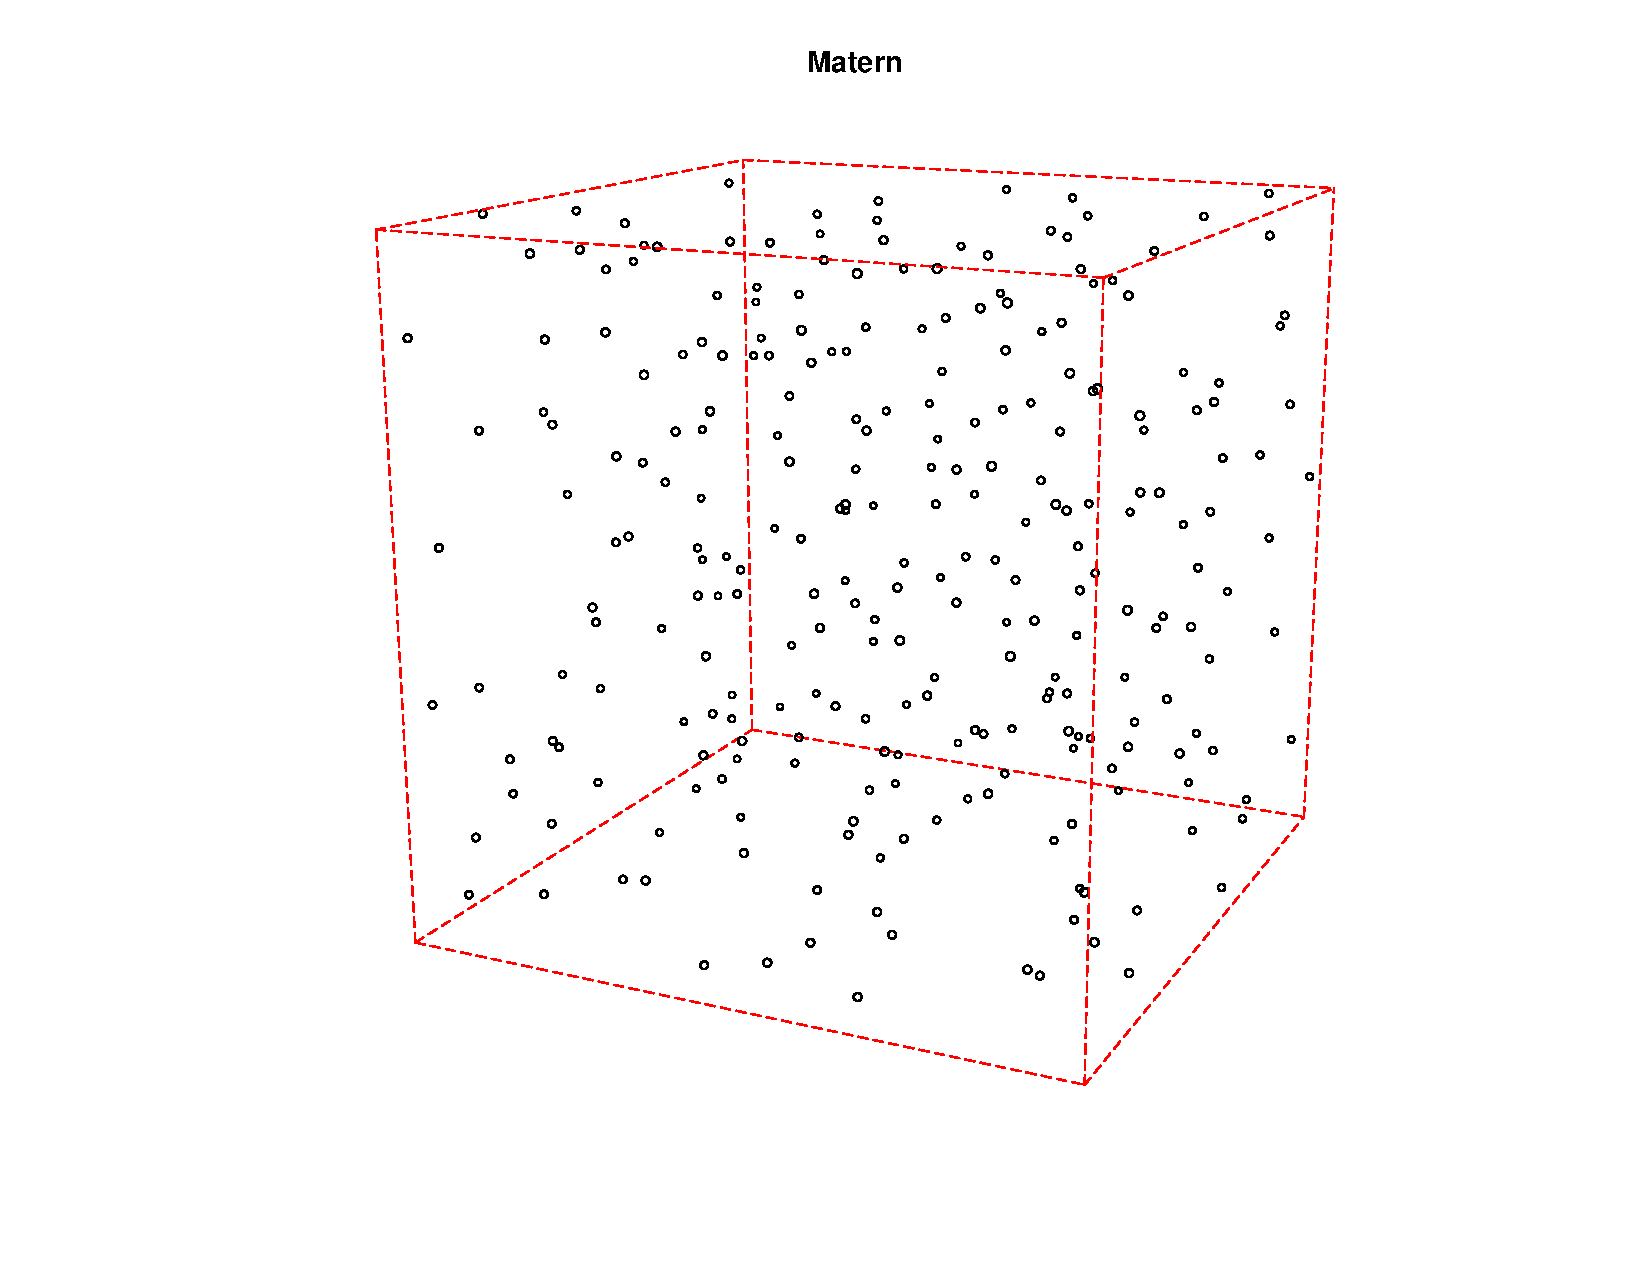
\includegraphics[width=0.9\textwidth]{PP_Matern_II_1000_0p1_275.pdf}
  \caption{Realization of a Matern II point process. Intensity 1000. Minimum distance 0.1. Number of points: 275.}
  \label{fig:matern2PP}

\vspace*{\floatsep}

    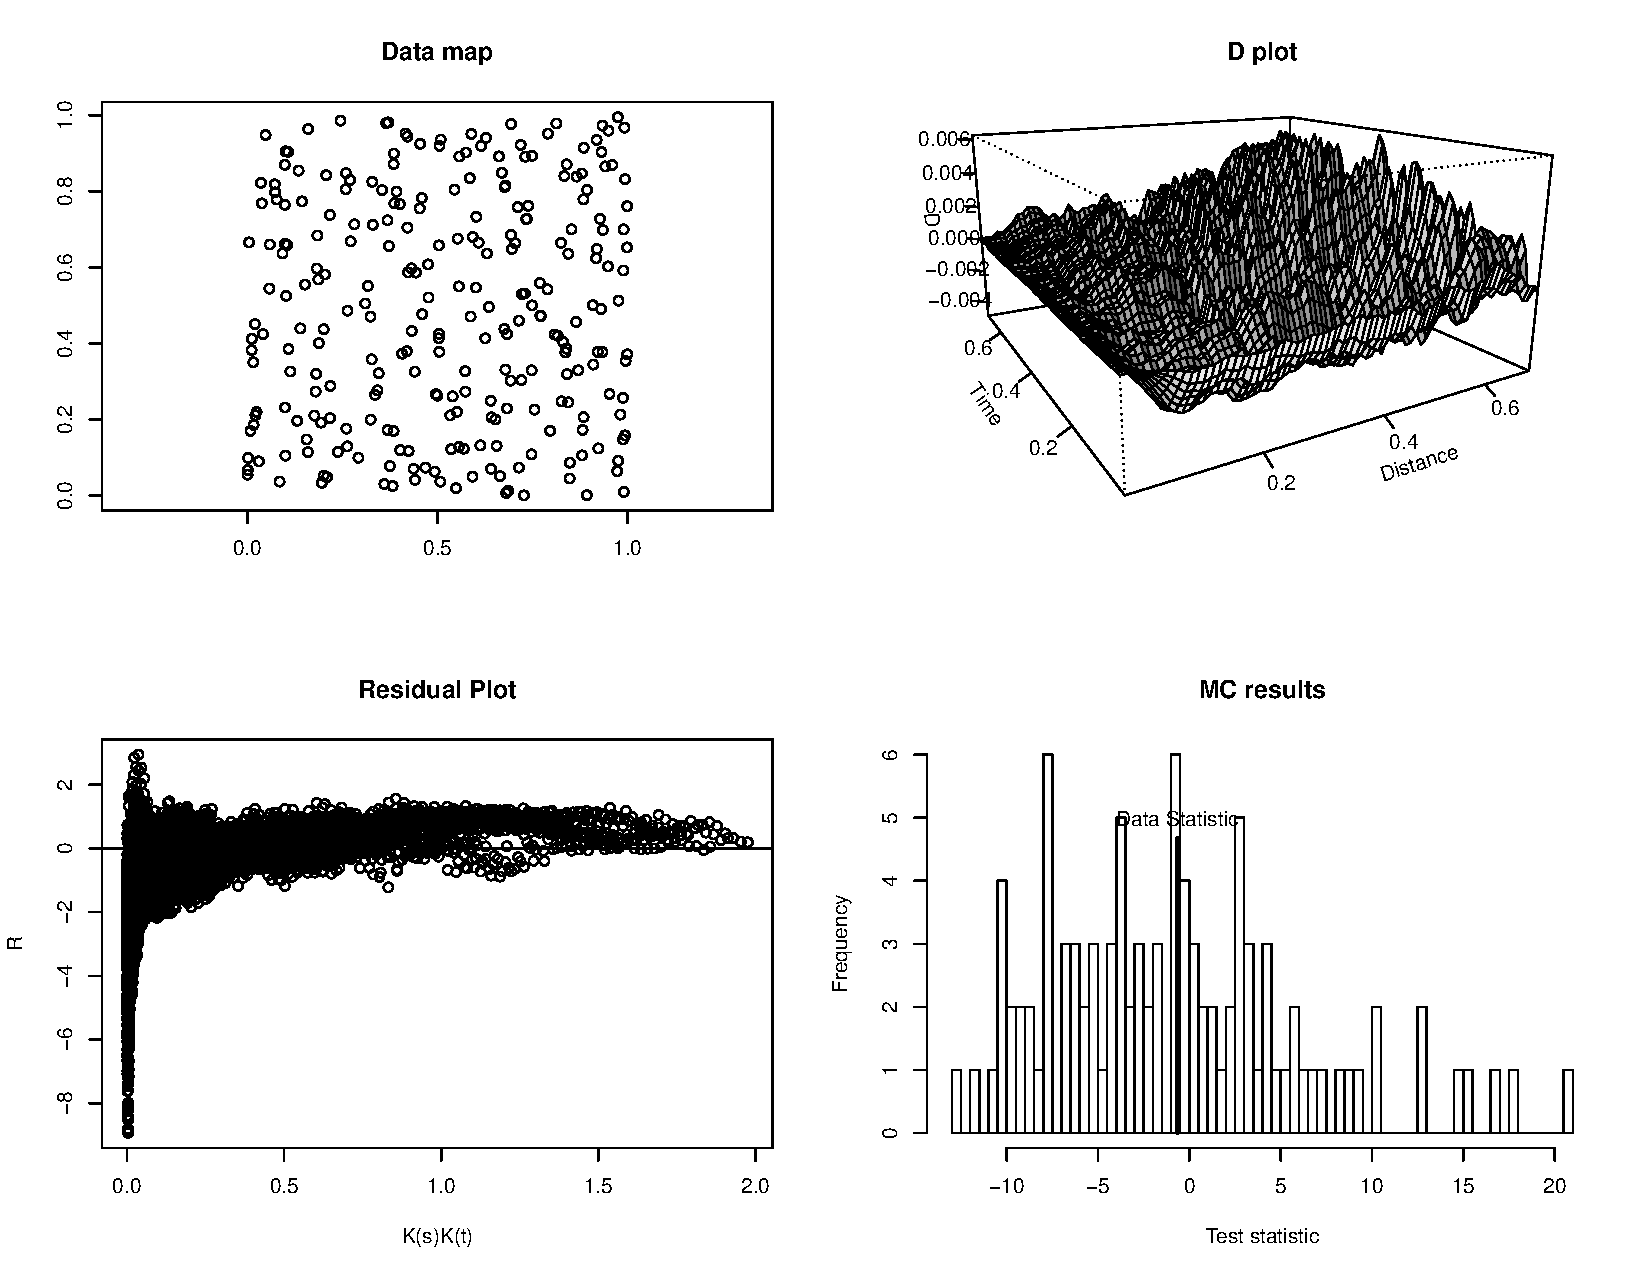
\includegraphics[width=0.9\textwidth]{diag_Matern_II_1000_0p1_275.pdf}
  \caption{Diagnostic plots for a realization of a Matern II point process.  Intensity 1000. Minimum distance 0.1. Number of points: 275.}
  \label{fig:matern2Diag}
\end{figure}





\section{Real data}




\begin{figure}[p]
  \centering
    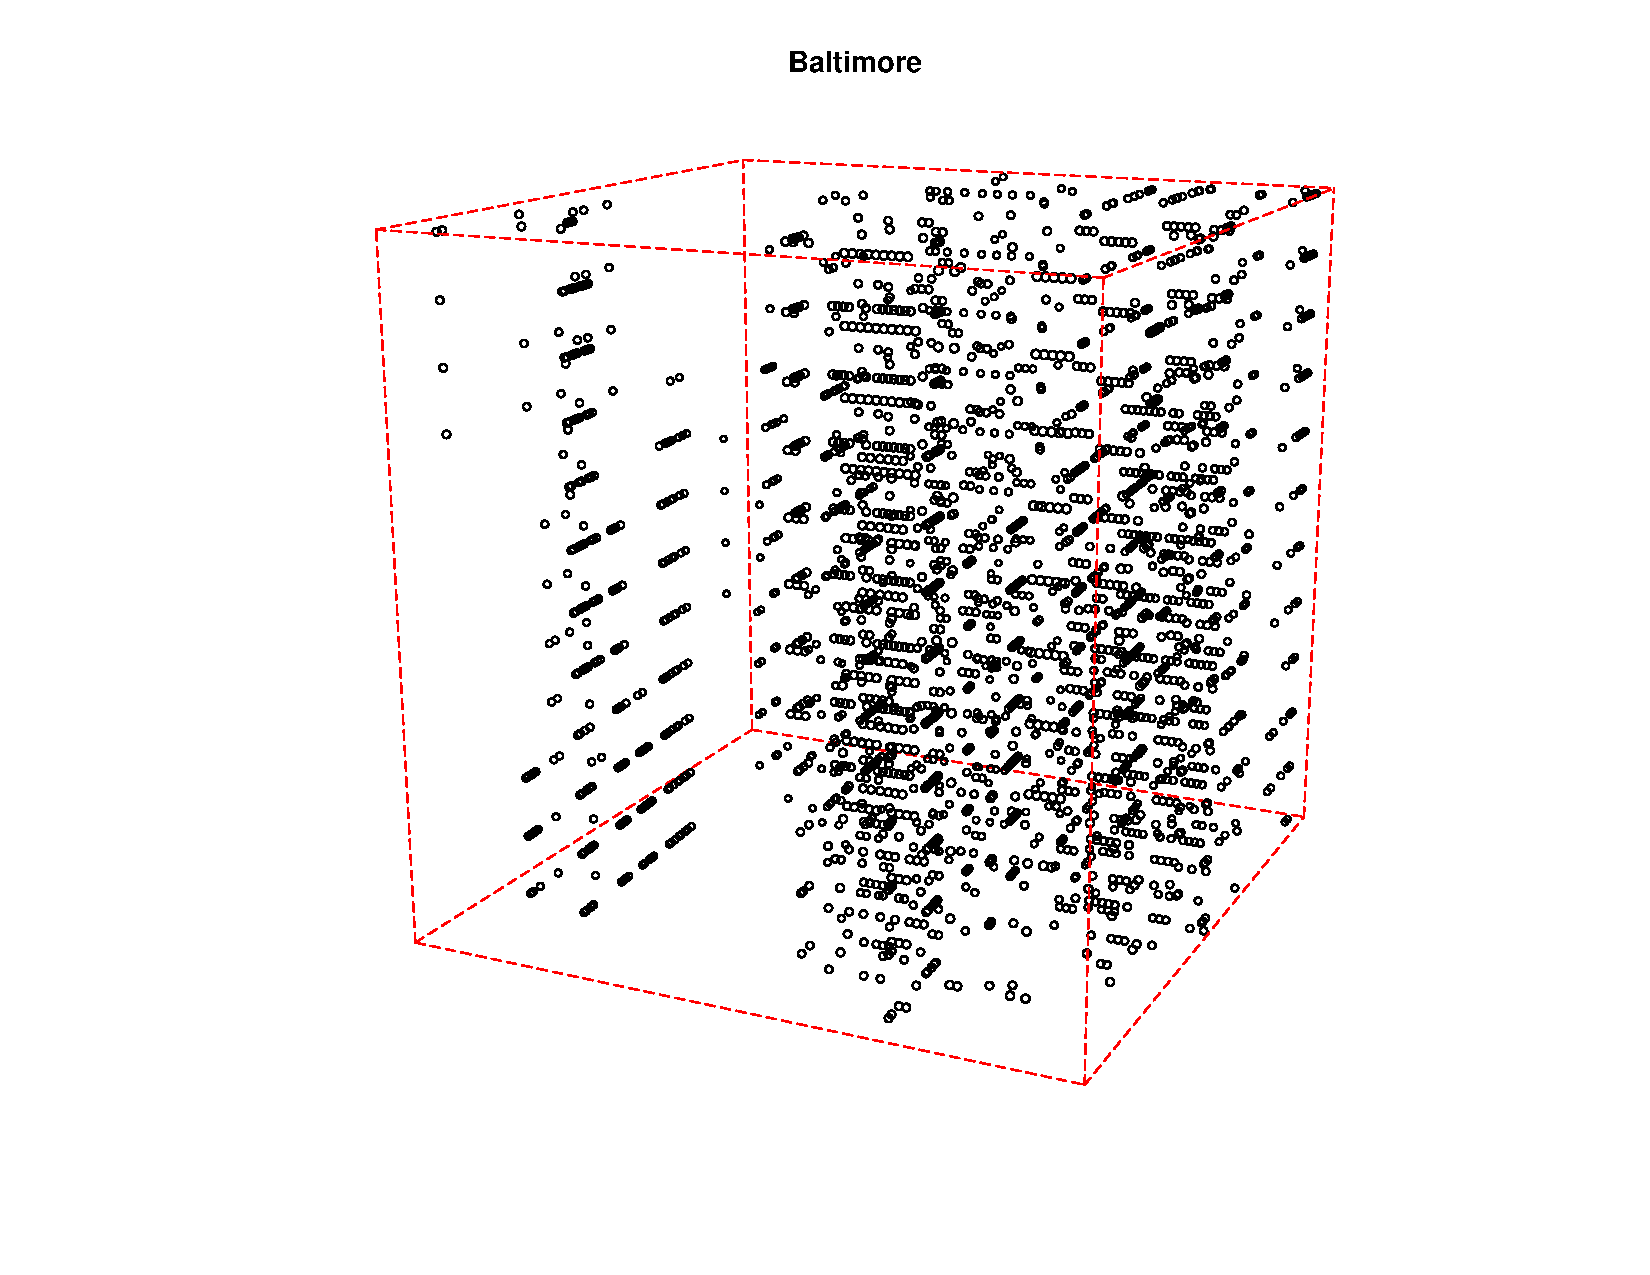
\includegraphics[width=0.9\textwidth]{PP_balt.pdf}
  \caption{Vacant flats represented as a spatio-temporal point process. First two dimension indicate location in coordinates, third dimension indicates year when flat was vacant. Number of points: 2538. }
  \label{fig:baltPP}

\vspace*{\floatsep}

    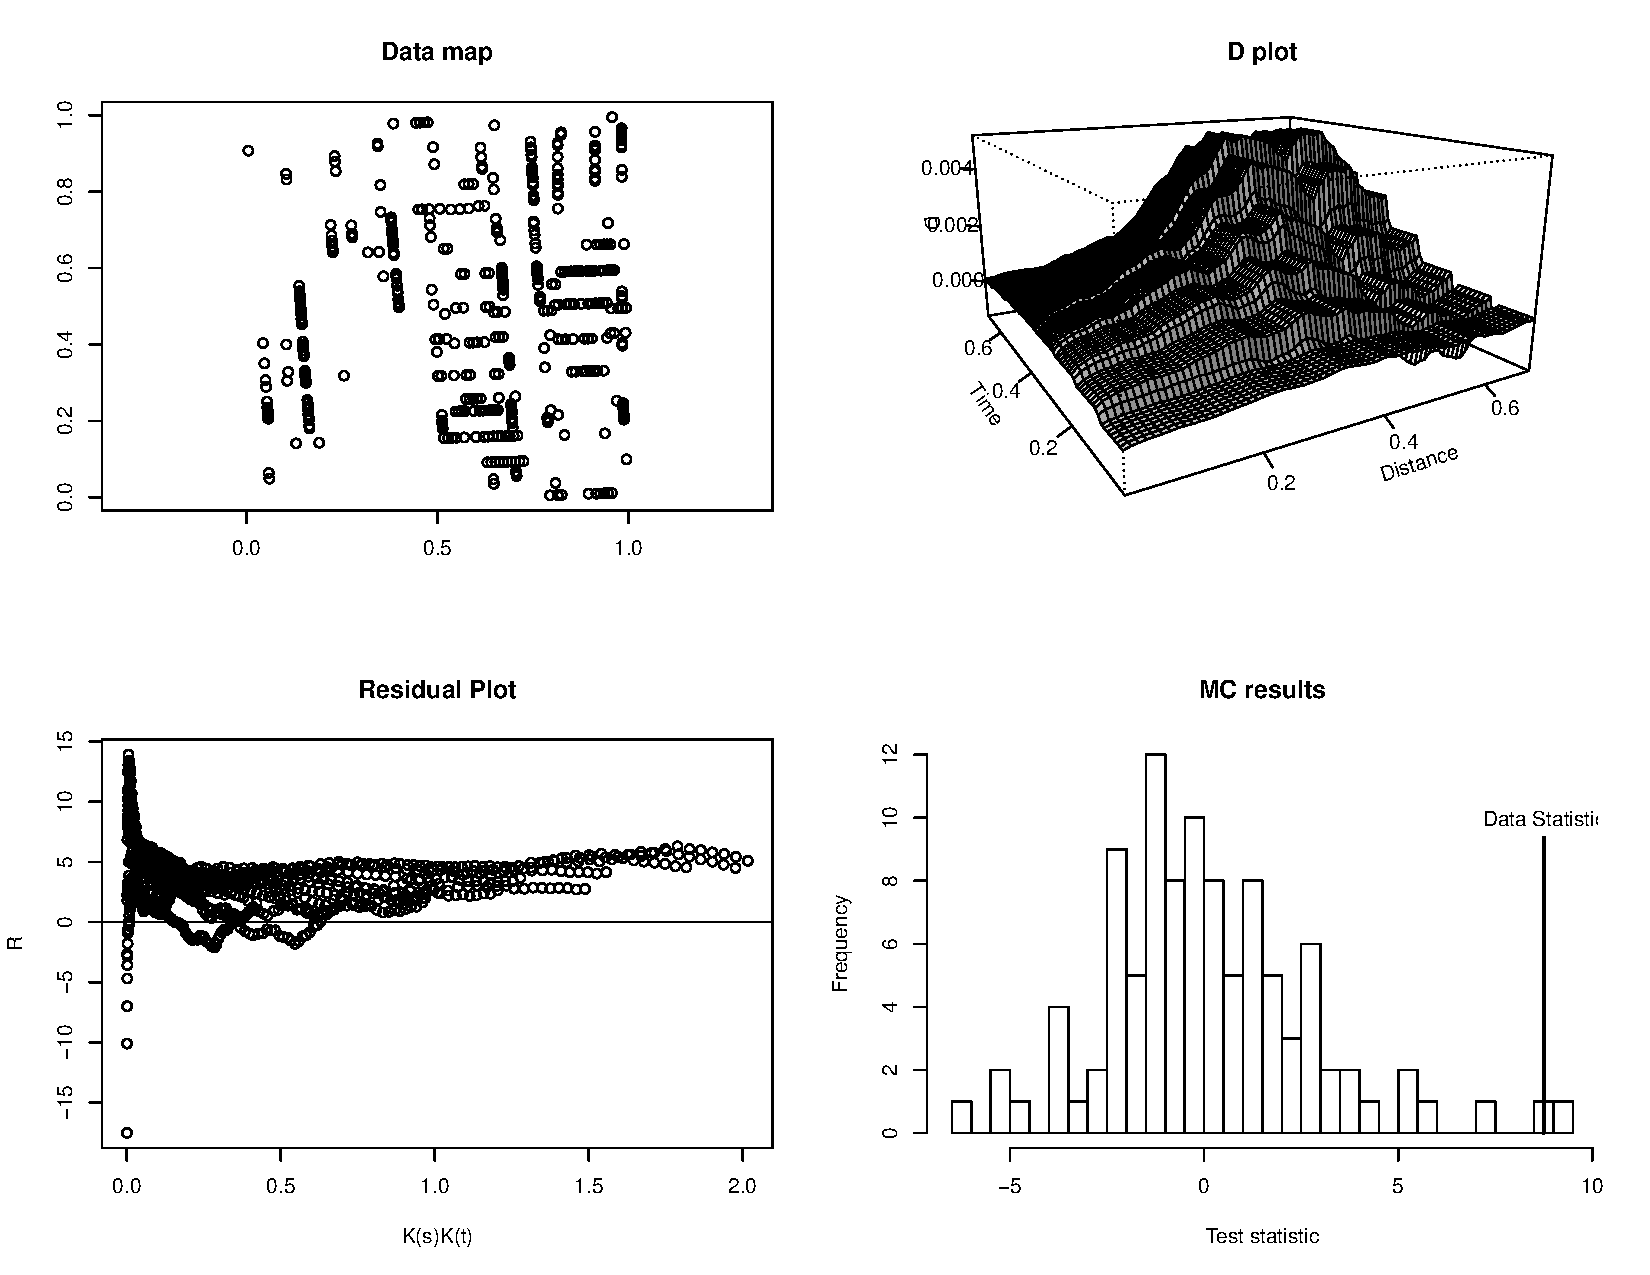
\includegraphics[width=0.9\textwidth]{diag_balt.pdf}
  \caption{Diagnostic plots for vacant flats represented as a spatio-temporal point process. Number of points: 2538. } 
  \label{fig:baltDiag}
\end{figure}



\begin{figure}[p]
  \centering
    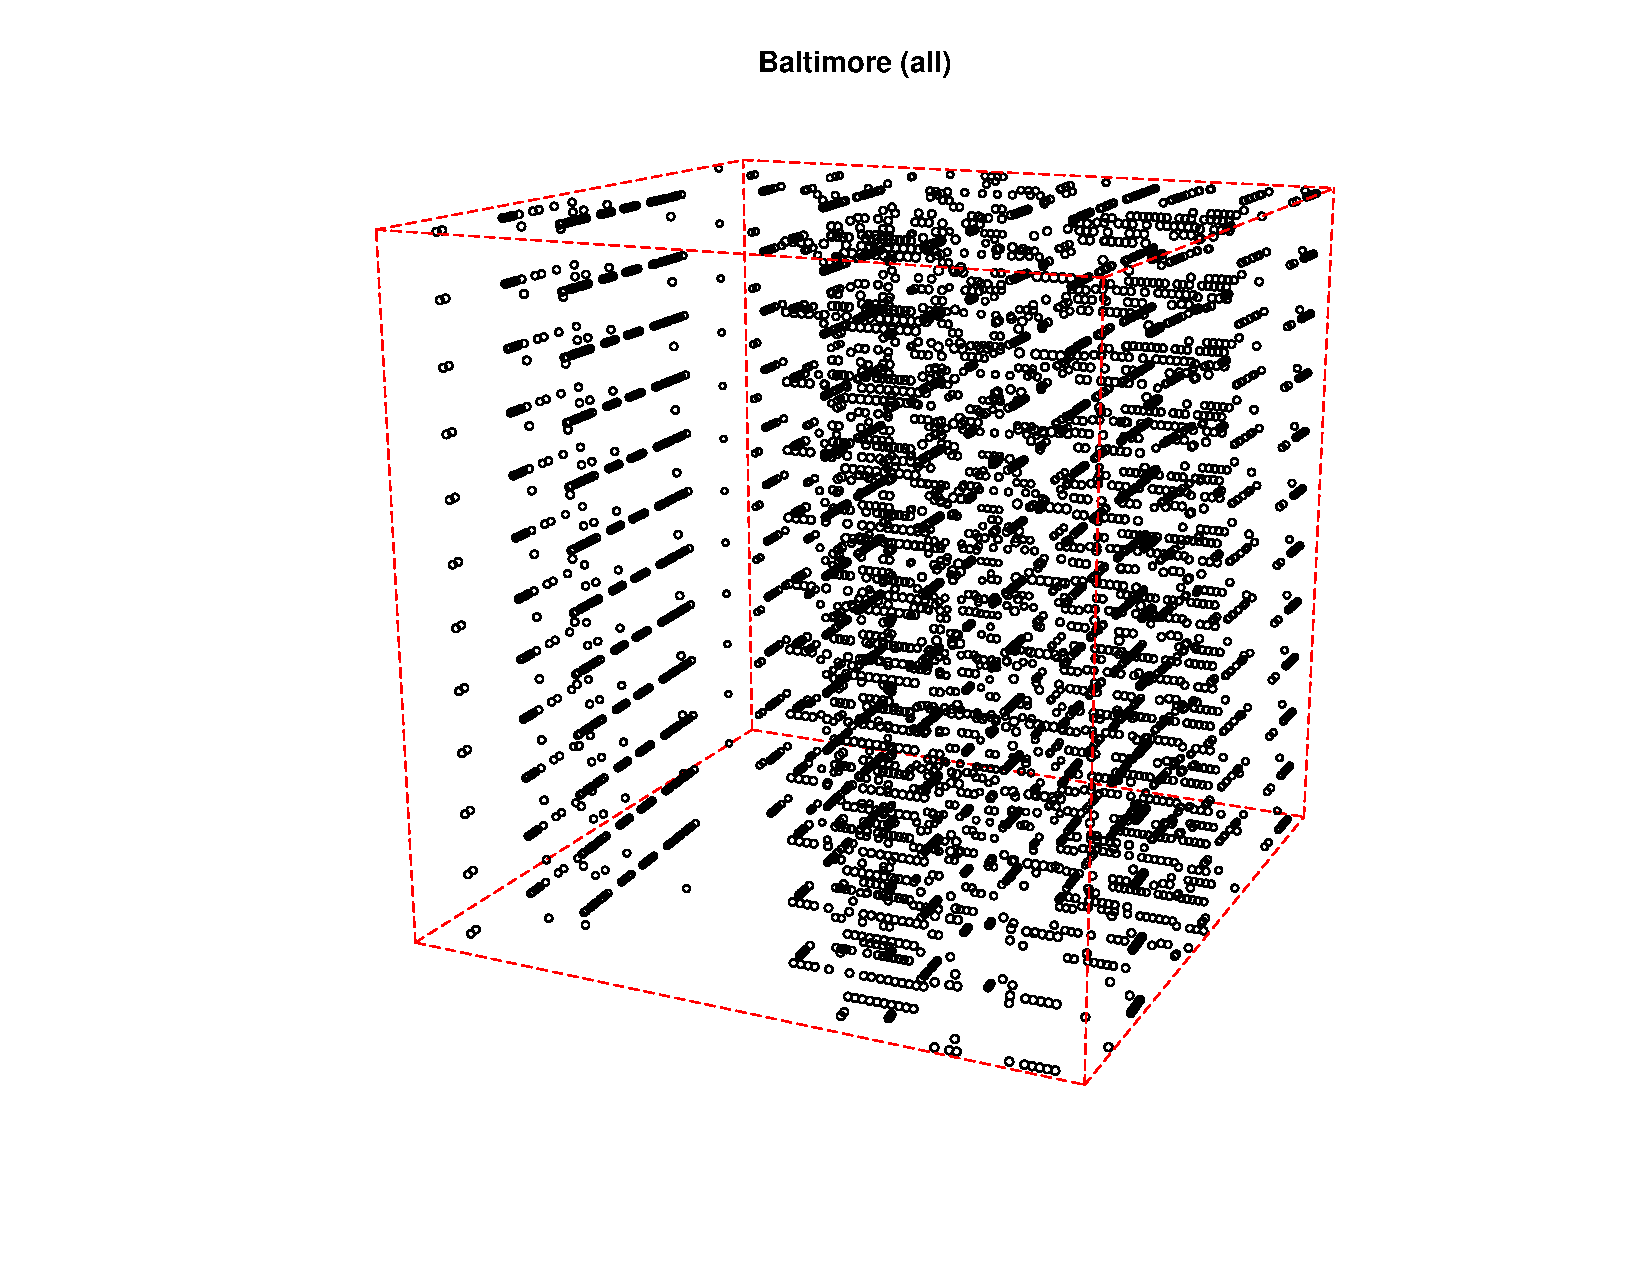
\includegraphics[width=0.9\textwidth]{PP_balt_full.pdf}
  \caption{Spatio-temporal point process composed of locations of all flats repeated in each year, regardless of whether it was vacant or not. Number of points: 4872. }
  \label{fig:baltallPP}

\vspace*{\floatsep}

    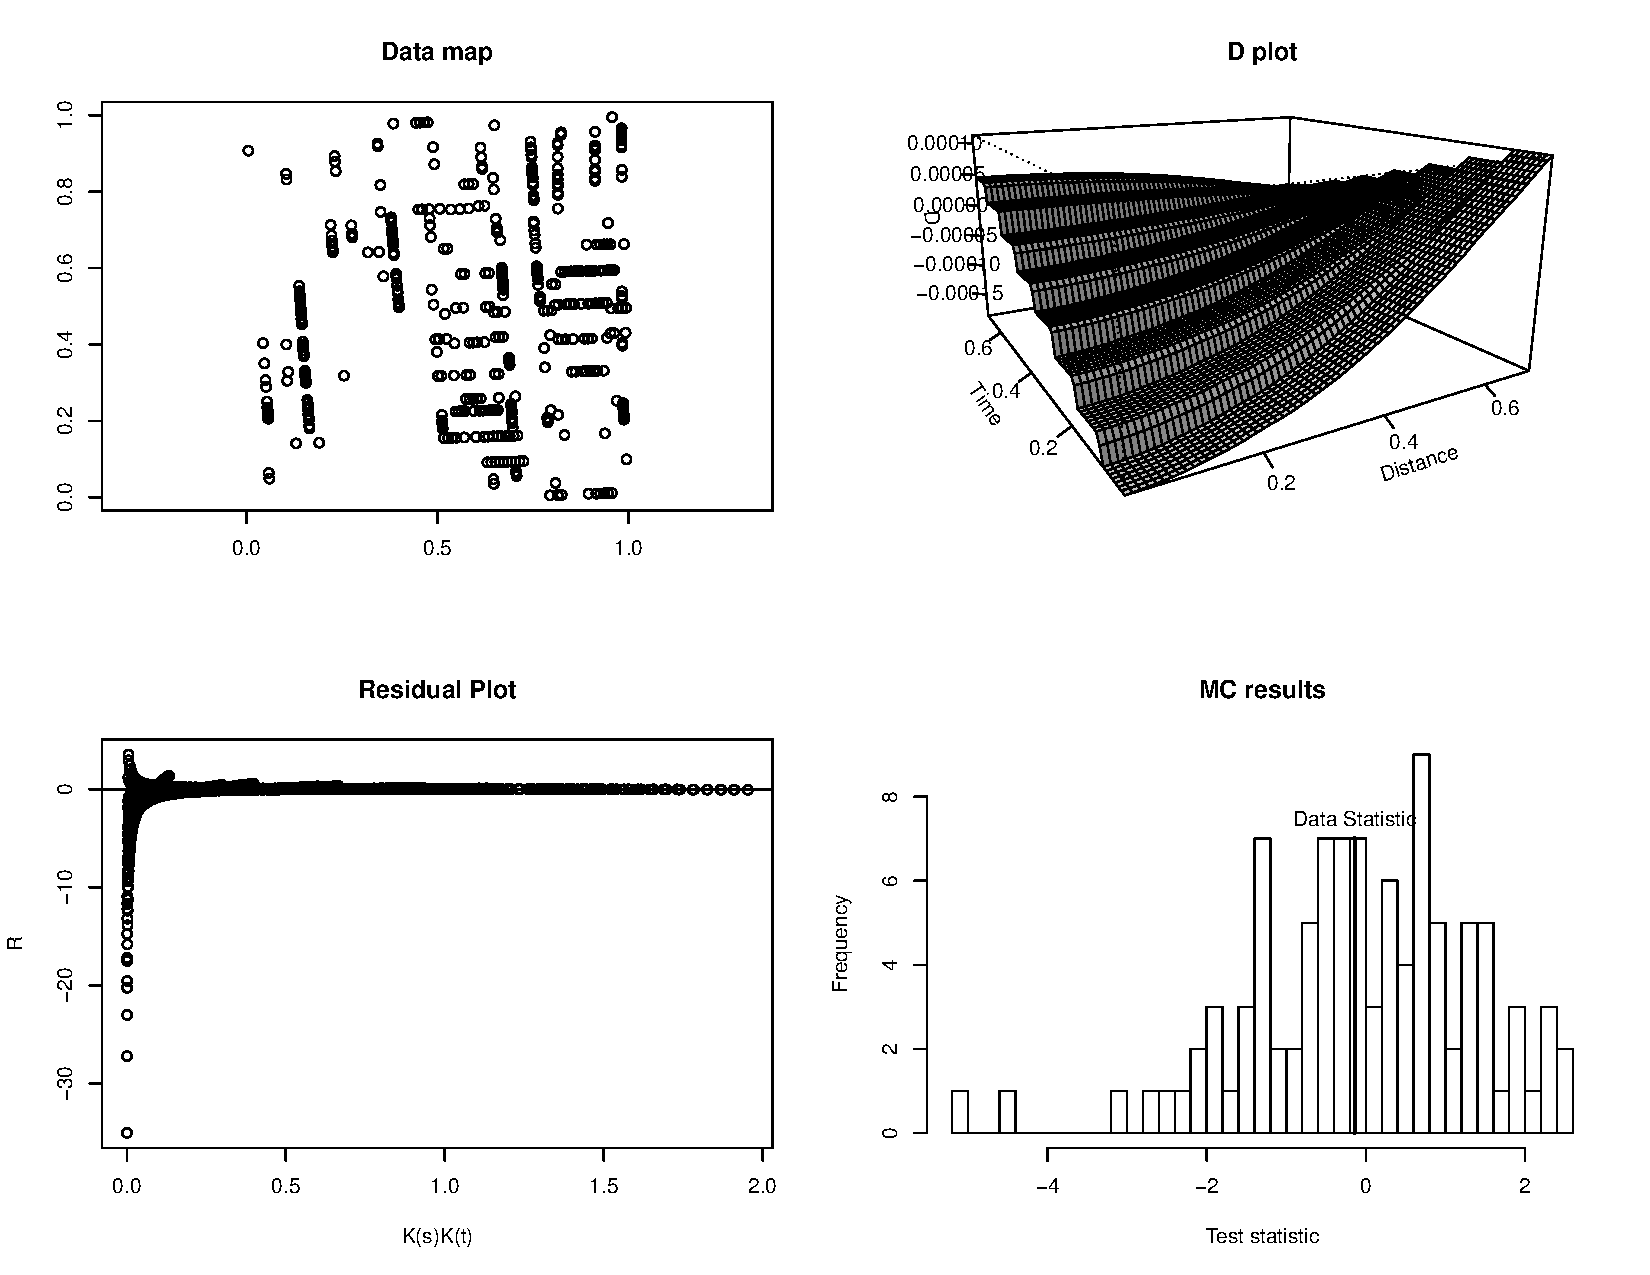
\includegraphics[width=0.9\textwidth]{diag_balt_full.pdf}
  \caption{Diagnostic plots for repeated locations of flats. Number of points: 4872. } 
  \label{fig:baltallDiag}
\end{figure}







\bibliography{bibliography}



\end{document}  %End of document.
